\documentclass[11pt]{article}
\usepackage{mathblatt}
% gesetzt von werkzeuge/setzer.py (Sorte selbst) aus dem Lernweg TCQ
% und den Bankzeilen; Muster bau/proben/2026-10-09/hypotenuse-muster.
\usepackage{enumitem}
\usepackage{adjustbox,varwidth}
\newgeometry{a4paper,margin=18mm,top=15mm,bottom=20mm,footskip=9mm}
\pagestyle{fancy}\fancyhf{}\renewcommand{\headrulewidth}{0pt}
\fancyfoot[L]{\footnotesize\color{mbgrau}TCQ \textperiodcentered{} Wachstum: linear oder exponentiell?}
\fancyfoot[R]{\footnotesize\color{mbgrau}\thepage}
\setlength{\parskip}{3pt}
\renewcommand{\kreuz}[1]{\mbox{$\square$\ #1}\quad}
\newcommand{\kreuzl}[1]{\par\hangindent1.4em\hangafter1\noindent$\square$\ #1}
\newcommand{\aufg}[3]{\par\noindent\makebox[0pt][r]{#3}\begin{minipage}[t]{\linewidth}#1\end{minipage}\par}
\newcommand{\aufgg}[4]{\par\noindent\makebox[0pt][r]{#4}\begin{minipage}[t]{0.6\linewidth}\vspace{0pt}#1\end{minipage}\hfill
  \begin{minipage}[t]{0.37\linewidth}\vspace{0pt}\centering #2\end{minipage}\par}
\newcommand{\nr}[1]{\makebox[7mm][l]{\textbf{#1}}}
\newcommand{\lsg}[3]{\par\noindent\begin{minipage}[t]{9mm}\textbf{#1}\end{minipage}%
  \begin{minipage}[t]{52mm}\raggedright\bfseries\boldmath #2\end{minipage}\hspace{3mm}%
  \begin{minipage}[t]{\dimexpr\linewidth-64mm\relax}\raggedright\small #3\end{minipage}\par\vspace{4pt}}
\newlength{\kr}
\makeatletter
\newcommand{\karomerk}[2]{\protected@write\@auxout{}{\string\karoseite{#1}{#2}{\thepage}}}
\newcommand{\karoseite}[3]{\expandafter\xdef\csname karo@#1@#2\endcsname{#3}}
\newcommand{\karohinweis}[3]{\karomerk{h}{#1}\ifcsname karo@k@#1\endcsname
  \ifnum\csname karo@k@#1\endcsname=0\csname karo@h@#1\endcsname\relax#2\else#3\fi
  \else#3\fi}
\makeatother
\begin{document}

\noindent{\LARGE\bfseries Wachstum: linear oder exponentiell?}\par\smallskip
\noindent{\small\color{mbgrau}Selbstlernheft Klasse 10 \textperiodcentered{} mit Lösungsheft \textperiodcentered{} Kennung TCQ}\par\medskip
\noindent\textbf{So nutzt du das Heft:} Lies im Abschnitt das Beispiel. Rechne dann die Aufgaben der Reihe nach und vergleiche jede sofort mit dem Lösungsheft. Kreuze „kann ich“ an, wenn du die letzte Aufgabe (\emph{Ziel}) allein schaffst.\par
\noindent Mehr Aufgaben zu einem Abschnitt: Kennung deinem Nachhilfelehrer schicken (z.\,B. „TCQ mehr B“).\par\medskip
{\arrayrulecolor{mbgrau}\renewcommand{\arraystretch}{1.3}
\noindent\begin{tabular}{|>{\bfseries}p{10mm}|p{112mm}|>{\raggedleft\arraybackslash}p{10mm}|>{\centering\arraybackslash}p{14mm}|}\hline
\rowcolor{black!8} & \textbf{Abschnitt} & \textbf{Seite} & \textbf{kann ich}\\\hline
A & An der Tabelle erkennen & \pageref{s:A} & $\square$\\\hline
B & Am Text erkennen & \pageref{s:B} & $\square$\\\hline
C & Den passenden Graphen finden & \pageref{s:C} & $\square$\\\hline
D & Wertepaare als Punkte eintragen & \pageref{s:D} & $\square$\\\hline
T & Probetest & \pageref{s:T} & $\square$\\\hline
\end{tabular}}\par\bigskip

\begin{tcolorbox}[colback=mbkasten,colframe=mbgrau,boxrule=0.5pt,arc=1mm,left=3mm,right=3mm,top=2mm,bottom=2mm,title={\bfseries Formel auf einen Blick},coltitle=black,colbacktitle=black!10]
\begin{minipage}[t]{0.58\linewidth}\vspace{0pt}
{\Large linear: \quad $y_{\text{neu}} = y_{\text{alt}} + d$ \par exponentiell: \quad $y_{\text{neu}} = y_{\text{alt}} \cdot q$}\par\medskip
In Worten: Linear kommt bei jedem Schritt derselbe Betrag dazu. Exponentiell wird bei jedem Schritt mit demselben Faktor malgenommen.\par\medskip
\textbf{So gehst du vor}\par
\nr{1}Tabelle: Differenzen und Quotienten bilden\par
\nr{2}Text: fester Betrag oder fester Prozentsatz?\par
\nr{3}Graph: Startwert auf der senkrechten Achse, Gerade oder Kurve\par
\nr{4}Punkte: Achsen gleichmäßig einteilen, eintragen, verbinden\par
\medskip
{\small Faktor über 1 heißt Zunahme, unter 1 Abnahme: $q = 1{,}1$ ist plus $10\,\%$, $q = 0{,}9$ ist minus $10\,\%$.}
\end{minipage}\hfill
\begin{minipage}[t]{0.38\linewidth}\vspace{2mm}\centering
\adjustbox{max width=\linewidth}{\begin{varwidth}{50cm}\begin{ksys}[xmin=0,xmax=4,ymin=0,ymax=800,xstep=0.5,ystep=100,karo=0.3,xlabel=Jahr,ylabel=€] \funktionab[3.0]{300*1.25^\x}{f}{0}{4} \gerade[3.9]{75}{300}{g} \funktionab[2.6]{45*\x^2}{h}{0}{4} \end{ksys}\end{varwidth}}
\end{minipage}
\end{tcolorbox}
\medskip\noindent\textbf{Typische Fehler – so nicht}\par\smallskip
\noindent\nr{$\times$}„Linear, weil jedes Jahr $5\,\%$.“ Gleicher Prozentsatz heißt gleicher Faktor: exponentiell.\par
\noindent\nr{$\times$}Den Graphen aus dem Ursprung genommen, obwohl der Startwert nicht $0$ ist.\par
\noindent\nr{$\times$}Zweimal $10\,\%$ zu $20\,\%$ addiert. Richtig: $1{,}1 \cdot 1{,}1 = 1{,}21$, also $21\,\%$.\par
\clearpage\label{s:A}\noindent\colorbox{black!12}{\makebox[10mm]{\Large\bfseries\strut A}}\hspace{3mm}{\Large\bfseries An der Tabelle erkennen}\par\smallskip
\noindent Gleiche Differenzen von Wert zu Wert: linear. Gleiche Quotienten von Wert zu Wert: exponentiell; der Quotient ist der Wachstumsfaktor $q$.\par\medskip
\noindent\textbf{Formel}\par\nopagebreak\noindent\hspace*{4mm}\begin{minipage}{\dimexpr\linewidth-4mm\relax}Differenz $=$ neuer Wert $-$ alter Wert \qquad Quotient $=$ neuer Wert $:$ alter Wert\end{minipage}\par\medskip
\noindent\textbf{Beispiel}\quad Die Tabelle zeigt die Zahl der Abonnenten eines Kanals. Wächst sie linear oder exponentiell? \adjustbox{max width=\linewidth}{\begin{varwidth}{50cm}\wertetabelle[400,440,484,532{,}4]{\text{Monat}}{\text{Abonnenten}}{0,1,2,3}\end{varwidth}}\par\smallskip
\noindent\par\noindent\hangindent6mm\hangafter1\makebox[6mm][l]{\textbf{1}}Differenzen: $440 - 400 = 40$; \ $484 - 440 = 44$; \ $532{,}4 - 484 = 48{,}4$. Nicht gleich, also nicht linear.\par\smallskip\par\noindent\hangindent6mm\hangafter1\makebox[6mm][l]{\textbf{2}}Quotienten: $440 : 400 = 1{,}1$; \ $484 : 440 = 1{,}1$; \ $532{,}4 : 484 = 1{,}1$. Immer gleich, also exponentiell.\par\smallskip\par\noindent\hangindent6mm\hangafter1\makebox[6mm][l]{\textbf{3}}Der Faktor $1{,}1$ heißt: jeden Monat $10\,\%$ mehr.\par\smallskip\par\noindent\hangindent6mm\hangafter1\makebox[6mm][l]{\textbf{4}}Antwort: Die Zahl wächst exponentiell mit dem Faktor $1{,}1$.\par\smallskip\par\medskip
\noindent\textbf{Aufgaben}\hspace{1em}{\small\color{mbgrau}\karohinweis{A}{Rechne unten im Karo.}{Rechne auf einem extra Blatt.} Vergleiche jede Aufgabe gleich mit dem Lösungsheft.}\par\smallskip
\aufg{\hangindent7mm\hangafter1\nr{1.}Die Tabelle zeigt, wie viel Wasser in einem Becken ist. Bilde die Differenzen. Wächst die Menge linear? \adjustbox{max width=\linewidth}{\begin{varwidth}{50cm}\wertetabelle[250,280,310,340]{\text{Minute}}{\text{Liter}}{0,1,2,3}\end{varwidth}}}{}{}
\medskip
\aufg{\hangindent7mm\hangafter1\nr{2.}Die Tabelle zeigt die Zahl der Fische in einem Teich. Bilde Differenzen und Quotienten. Wächst die Zahl linear oder exponentiell? Gib den Faktor und den Prozentsatz an. \adjustbox{max width=\linewidth}{\begin{varwidth}{50cm}\wertetabelle[320,400,500,625]{\text{Jahr}}{\text{Fische}}{0,1,2,3}\end{varwidth}}}{}{}
\medskip
\aufg{\hangindent7mm\hangafter1\nr{3.}Die Tabelle zeigt den Wert eines Motorrollers. Linear oder exponentiell? Gib an, um wie viel Prozent der Wert jedes Jahr abnimmt. \adjustbox{max width=\linewidth}{\begin{varwidth}{50cm}\wertetabelle[2000,1600,1280,1024]{\text{Jahr}}{\text{Wert in €}}{0,1,2,3}\end{varwidth}}}{}{}
\medskip
\aufg{\hangindent7mm\hangafter1\nr{4.}Nach einer Spritze wird ein Medikament im Blut abgebaut. Die Tabelle zeigt die Menge. Kreuze die zwei richtigen Aussagen an. \adjustbox{max width=\linewidth}{\begin{varwidth}{50cm}\wertetabelle[300,270,243,218{,}7]{\text{Stunde}}{\text{Menge in mg}}{0,1,2,3}\end{varwidth}}\par\smallskip\leftskip7mm \kreuzl{Jede Stunde nimmt die Menge um $30$ mg ab.}\kreuzl{Jede Stunde nimmt die Menge um $10\,\%$ ab.}\kreuzl{Die Menge nimmt linear ab.}\kreuzl{Die Abnahme in mg wird jede Stunde kleiner.}}{}{{\scriptsize\color{mbgrau}Ziel\hspace{2mm}}}
\medskip
\par\vspace{3mm}\setlength{\kr}{\dimexpr\pagegoal-\pagetotal-10mm\relax}%
\ifdim\kr>12mm\karomerk{k}{A}\noindent{\scriptsize\color{mbgrau}Platz zum Rechnen}\par\nointerlineskip\vspace{1mm}\noindent
\begin{tikzpicture}\clip (0,0) rectangle ({\linewidth-0.5mm},\kr);\draw[black!16,line width=0.3pt,step=5mm] (0,0) grid (\linewidth,\kr);\end{tikzpicture}\fi\par
\clearpage\label{s:B}\noindent\colorbox{black!12}{\makebox[10mm]{\Large\bfseries\strut B}}\hspace{3mm}{\Large\bfseries Am Text erkennen}\par\smallskip
\noindent Ein fester Betrag je Schritt (Euro, Liter, Zentimeter) bedeutet linear. Ein fester Prozentsatz, „das Doppelte“ oder „die Hälfte“ bedeutet exponentiell: Dann wird der Zuwachs von Schritt zu Schritt größer, die Abnahme kleiner.\par\medskip
\noindent\textbf{Formel}\par\nopagebreak\noindent\hspace*{4mm}\begin{minipage}{\dimexpr\linewidth-4mm\relax}Zunahme um $p\,\%$: \ $q = 1 + \frac{p}{100}$ \qquad Abnahme um $p\,\%$: \ $q = 1 - \frac{p}{100}$\end{minipage}\par\medskip
\noindent\textbf{Beispiel}\quad Auf einem Konto liegen $800\,€$. Jedes Jahr kommen $5\,\%$ Zinsen dazu. Ben sagt: „Das sind jedes Jahr $40\,€$ mehr.“ Hat er recht?\par\smallskip
\noindent\par\noindent\hangindent6mm\hangafter1\makebox[6mm][l]{\textbf{1}}„$5\,\%$ jedes Jahr“: gleicher Faktor $1{,}05$, also exponentiell. („$40\,€$ jedes Jahr“ wäre linear.)\par\smallskip\par\noindent\hangindent6mm\hangafter1\makebox[6mm][l]{\textbf{2}}Zwei Jahre rechnen, jedes Mal vom letzten Wert aus: \ $800 \cdot 1{,}05 = 840$; \ $840 \cdot 1{,}05 = 882$.\par\smallskip\par\noindent\hangindent6mm\hangafter1\makebox[6mm][l]{\textbf{3}}Zuwächse vergleichen: $840 - 800 = 40$; \ $882 - 840 = 42$. Der Zuwachs wird größer.\par\smallskip\par\noindent\hangindent6mm\hangafter1\makebox[6mm][l]{\textbf{4}}Antwort: Nein. Nur im ersten Jahr sind es $40\,€$, danach mehr.\par\smallskip\par\medskip
\noindent\textbf{Aufgaben}\hspace{1em}{\small\color{mbgrau}\karohinweis{B}{Rechne unten im Karo.}{Rechne auf einem extra Blatt.} Vergleiche jede Aufgabe gleich mit dem Lösungsheft.}\par\smallskip
\aufg{\hangindent7mm\hangafter1\nr{1.}Linear oder exponentiell? Schreib L oder E und dazu „zu“ oder „ab“. \par a) Eine Kerze wird jede Stunde $2$ cm kürzer. \par b) Die Zahl der Follower wächst jede Woche um $8\,\%$. \par c) Ein Handy verliert jedes Jahr $30\,\%$ seines Werts. \par d) In ein Becken laufen jede Minute $15$ Liter.}{}{}
\medskip
\aufg{\hangindent7mm\hangafter1\nr{2.}Ein Auto kostet neu $24\,000\,€$. Es verliert jedes Jahr $15\,\%$ seines Werts. Tim sagt: „Das Auto verliert jedes Jahr $3\,600\,€$.“ Rechne zwei Jahre. Hat Tim recht?}{}{}
\medskip
\aufg{\hangindent7mm\hangafter1\nr{3.}Eine App hat $400$ Nutzer. Die Zahl steigt zwei Monate lang um je $50\,\%$. Ali sagt: „Dann sind es doppelt so viele.“ Rechne nach. Hat Ali recht?}{}{}
\medskip
\aufg{\hangindent7mm\hangafter1\nr{4.}Für einen Ferienjob gibt es zwei Angebote. In Woche $1$ zahlen beide $40\,€$. Angebot A: danach jede Woche $8\,€$ mehr. Angebot B: danach jede Woche $15\,\%$ mehr. Welches Angebot zahlt in Woche $4$ mehr? In welcher Woche zahlt B zum ersten Mal mehr als A?}{}{{\scriptsize\color{mbgrau}Ziel\hspace{2mm}}}
\medskip
\par\vspace{3mm}\setlength{\kr}{\dimexpr\pagegoal-\pagetotal-10mm\relax}%
\ifdim\kr>12mm\karomerk{k}{B}\noindent{\scriptsize\color{mbgrau}Platz zum Rechnen}\par\nointerlineskip\vspace{1mm}\noindent
\begin{tikzpicture}\clip (0,0) rectangle ({\linewidth-0.5mm},\kr);\draw[black!16,line width=0.3pt,step=5mm] (0,0) grid (\linewidth,\kr);\end{tikzpicture}\fi\par
\clearpage\label{s:C}\noindent\colorbox{black!12}{\makebox[10mm]{\Large\bfseries\strut C}}\hspace{3mm}{\Large\bfseries Den passenden Graphen finden}\par\smallskip
\noindent Linear ergibt eine Gerade. Exponentiell ergibt eine Kurve: bei Zunahme immer steiler, bei Abnahme immer flacher. Der Graph beginnt beim Startwert auf der senkrechten Achse.\par\medskip
\noindent\textbf{Formel}\par\nopagebreak\noindent\hspace*{4mm}\begin{minipage}{\dimexpr\linewidth-4mm\relax}Startwert $a$ \ $\to$ \ Punkt $(0\,|\,a)$ \qquad gleicher Betrag \ $\to$ \ Gerade \qquad gleicher Faktor \ $\to$ \ Kurve\end{minipage}\par\medskip
\noindent\textbf{Beispiel}\quad Auf einem Konto liegen zu Beginn $300\,€$. Das Guthaben wächst jedes Jahr um $25\,\%$. Welcher Graph passt?\par\smallskip
\noindent\begin{minipage}[t]{0.6\linewidth}\vspace{0pt}\par\noindent\hangindent6mm\hangafter1\makebox[6mm][l]{\textbf{1}}Startwert $300\,€$: Der Graph beginnt bei $(0\,|\,300)$. $h$ beginnt bei $0$, passt nicht.\par\smallskip\par\noindent\hangindent6mm\hangafter1\makebox[6mm][l]{\textbf{2}}„$25\,\%$ jedes Jahr“: gleicher Faktor, also eine Kurve. $g$ ist eine Gerade, passt nicht.\par\smallskip\par\noindent\hangindent6mm\hangafter1\makebox[6mm][l]{\textbf{3}}$f$ bleibt: beginnt bei $300$ und wird immer steiler. Bei Abnahme fällt die Kurve und wird flacher.\par\smallskip\par\noindent\hangindent6mm\hangafter1\makebox[6mm][l]{\textbf{4}}Antwort: Graph $f$.\par\smallskip\end{minipage}\hfill
\begin{minipage}[t]{0.37\linewidth}\vspace{0pt}\centering \adjustbox{max width=\linewidth}{\begin{varwidth}{50cm}\begin{ksys}[xmin=0,xmax=4,ymin=0,ymax=800,xstep=0.5,ystep=100,karo=0.3,xlabel=Jahr,ylabel=€] \funktionab[3.0]{300*1.25^\x}{f}{0}{4} \gerade[3.9]{75}{300}{g} \funktionab[2.6]{45*\x^2}{h}{0}{4} \end{ksys}\end{varwidth}}\end{minipage}\par\medskip
\noindent\textbf{Aufgaben}\hspace{1em}{\small\color{mbgrau}\karohinweis{C}{Rechne unten im Karo.}{Rechne auf einem extra Blatt.} Vergleiche jede Aufgabe gleich mit dem Lösungsheft.}\par\smallskip
\aufgg{\hangindent7mm\hangafter1\nr{1.}Das Koordinatensystem zeigt drei Graphen. Schreib zu jedem: Gerade oder Kurve? Steigt er oder fällt er? Wo beginnt er?}{\begin{tikzpicture}\node[inner sep=0pt]{\begin{ksys}[xmin=0,xmax=5,ymin=0,ymax=450,xstep=0.5,ystep=50,karo=0.28,xlabel=Jahr,ylabel=Wert] \funktionab{400*0.8^\x}{}{0}{5} \gerade{40}{100}{} \funktionab{50*1.4^\x}{}{0}{5} \node[anchor=south west,inner sep=2pt,font=\small] at (0.8,334) {$g$};\node[anchor=south east,inner sep=2pt,font=\small] at (4.5,280) {$f$};\node[anchor=north west,inner sep=2pt,font=\small] at (2,98) {$h$}; \end{ksys}};\end{tikzpicture}}{}{}
\medskip
\aufgg{\hangindent7mm\hangafter1\nr{2.}Ein Tank enthält $150$ Liter Wasser. Jede Minute laufen $30$ Liter dazu. Kreuze den passenden Graphen an und begründe in einem Satz.\par\smallskip\leftskip7mm \kreuz{$f$}\ \kreuz{$g$}\par\kreuz{$h$}}{\adjustbox{max width=\linewidth}{\begin{varwidth}{50cm}\begin{ksys}[xmin=0,xmax=6,ymin=0,ymax=600,xstep=0.5,ystep=100,karo=0.28,xlabel=Minute,ylabel=Liter] \funktionab[5.2]{150*1.25^\x}{f}{0}{6} \gerade[5.5]{30}{150}{g} \gerade[4.5]{30}{0}{h} \end{ksys}\end{varwidth}}}{}{}
\medskip
\aufgg{\hangindent7mm\hangafter1\nr{3.}Ein Fitnessstudio hat $400$ Mitglieder. Jedes Jahr kommen $12\,\%$ dazu. Kreuze den Graphen an, der die Zahl der Mitglieder zeigt. Begründe für die beiden anderen Graphen, warum sie nicht passen.\par\smallskip\leftskip7mm \kreuz{$f$}\ \kreuz{$g$}\par\kreuz{$h$}}{\begin{tikzpicture}\node[inner sep=0pt]{\begin{ksys}[xmin=0,xmax=8,ymin=0,ymax=1000,xstep=1,ystep=100,karo=0.28,xlabel=Jahr,ylabel=Mitglieder] \gerade{48}{400}{} \funktionab{400*1.12^\x}{}{0}{8} \funktionab{12*\x^2}{}{0}{8} \node[anchor=north west,inner sep=2pt,font=\small] at (2,496) {$f$};\node[anchor=south east,inner sep=2pt,font=\small] at (6.3,814) {$g$};\node[anchor=north west,inner sep=2pt,font=\small] at (6,432) {$h$}; \end{ksys}};\end{tikzpicture}}{}{{\scriptsize\color{mbgrau}Ziel\hspace{2mm}}}
\medskip
\par\vspace{3mm}\setlength{\kr}{\dimexpr\pagegoal-\pagetotal-10mm\relax}%
\ifdim\kr>12mm\karomerk{k}{C}\noindent{\scriptsize\color{mbgrau}Platz zum Rechnen}\par\nointerlineskip\vspace{1mm}\noindent
\begin{tikzpicture}\clip (0,0) rectangle ({\linewidth-0.5mm},\kr);\draw[black!16,line width=0.3pt,step=5mm] (0,0) grid (\linewidth,\kr);\end{tikzpicture}\fi\par
\clearpage\label{s:D}\noindent\colorbox{black!12}{\makebox[10mm]{\Large\bfseries\strut D}}\hspace{3mm}{\Large\bfseries Wertepaare als Punkte eintragen}\par\smallskip
\noindent Teile jede Achse gleichmäßig ein, sodass der größte Wert passt. Trage die Punkte ein und verbinde sie mit einer glatten Kurve.\par\medskip
\noindent\textbf{Formel}\par\nopagebreak\noindent\hspace*{4mm}\begin{minipage}{\dimexpr\linewidth-4mm\relax}größter Wert \ $\to$ \ Schritt je Kästchen (1, 2, 5, 10, 20, \dots) \ $\to$ \ beschriften \ $\to$ \ Punkte \ $\to$ \ Kurve\end{minipage}\par\medskip
\noindent\textbf{Beispiel}\quad Die Tabelle zeigt die Fläche eines Schimmelflecks. Stelle die Werte in einem Koordinatensystem dar. \adjustbox{max width=\linewidth}{\begin{varwidth}{50cm}\wertetabelle[7,14,28,56,112]{\text{Tag}}{\text{Fläche in cm²}}{0,1,2,3,4}\end{varwidth}}\par\smallskip
\noindent\begin{minipage}[t]{0.6\linewidth}\vspace{0pt}\par\noindent\hangindent6mm\hangafter1\makebox[6mm][l]{\textbf{1}}Größter Wert: $112$. Die senkrechte Achse muss darüber reichen.\par\smallskip\par\noindent\hangindent6mm\hangafter1\makebox[6mm][l]{\textbf{2}}1 Kästchen $= 20$ cm² (bis $120$), waagerecht 1 Kästchen $=$ 1 Tag. Achsen beschriften.\par\smallskip\par\noindent\hangindent6mm\hangafter1\makebox[6mm][l]{\textbf{3}}Punkte eintragen: $(0\,|\,7)$ gut ein Drittel Kästchen hoch, $(1\,|\,14)$ knapp drei Viertel, dann $(2\,|\,28)$, $(3\,|\,56)$, $(4\,|\,112)$.\par\smallskip\par\noindent\hangindent6mm\hangafter1\makebox[6mm][l]{\textbf{4}}Frei Hand verbinden, ohne Ecken. Die Kurve wird steiler: exponentiell.\par\smallskip\end{minipage}\hfill
\begin{minipage}[t]{0.37\linewidth}\vspace{0pt}\centering \adjustbox{max width=\linewidth}{\begin{varwidth}{50cm}\begin{ksys}[xmin=0,xmax=5,ymin=0,ymax=120,xstep=1,ystep=20,karo=0.32,xlabel=Tag,ylabel=cm$^2$] \punkt{0}{7}{} \punkt{1}{14}{} \punkt{2}{28}{} \punkt{3}{56}{} \punkt{4}{112}{} \funktionab{7*2^\x}{}{0}{4} \end{ksys}\end{varwidth}}\end{minipage}\par\medskip
\noindent\textbf{Aufgaben}\hspace{1em}{\small\color{mbgrau}\karohinweis{D}{Rechne unten im Karo.}{Rechne auf einem extra Blatt.} Vergleiche jede Aufgabe gleich mit dem Lösungsheft.}\par\smallskip
\aufgg{\hangindent7mm\hangafter1\nr{1.}Die Tabelle zeigt die Mitglieder eines Online-Clubs. Trage die Wertepaare als Punkte in das Koordinatensystem ein. \adjustbox{max width=\linewidth}{\begin{varwidth}{50cm}\wertetabelle[10,20,40,80]{\text{Monat}}{\text{Mitglieder}}{0,1,2,3}\end{varwidth}}}{\adjustbox{max width=\linewidth}{\begin{varwidth}{50cm}\begin{ksys}[xmin=0,xmax=5,ymin=0,ymax=80,xstep=1,ystep=10,karo=0.3,xlabel=Monat,ylabel=Mitglieder]  \end{ksys}\end{varwidth}}}{}{}
\medskip
\aufgg{\hangindent7mm\hangafter1\nr{2.}Die Tabelle zeigt die Zahl der Hefezellen (in Tausend). Trage die Punkte ein und verbinde sie zu einer Kurve. \adjustbox{max width=\linewidth}{\begin{varwidth}{50cm}\wertetabelle[40,56,78,110,154]{\text{Stunde}}{\text{Zellen}}{0,1,2,3,4}\end{varwidth}}}{\adjustbox{max width=\linewidth}{\begin{varwidth}{50cm}\begin{ksys}[xmin=0,xmax=5,ymin=0,ymax=160,xstep=1,ystep=20,karo=0.3,xlabel=Stunde,ylabel=Zellen]  \end{ksys}\end{varwidth}}}{}{}
\medskip
\aufgg{\hangindent7mm\hangafter1\nr{3.}Die Tabelle zeigt die Downloads einer App (in Tausend). Teile die Achsen selbst ein, beschrifte sie und trage die Punkte ein. Wachsen die Downloads linear oder exponentiell? Begründe am Graphen. \adjustbox{max width=\linewidth}{\begin{varwidth}{50cm}\wertetabelle[8,12,18,27,40{,}5]{\text{Woche}}{\text{Downloads}}{0,1,2,3,4}\end{varwidth}}}{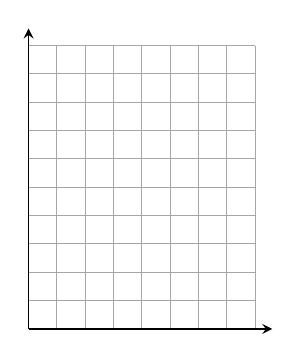
\begin{tikzpicture}[x=0.36cm,y=0.36cm]\draw[black!35,line width=0.4pt] (0,0) grid[step=1] (8,10);\draw[-stealth,line width=0.6pt] (0,0) -- (8.6,0);\draw[-stealth,line width=0.6pt] (0,0) -- (0,10.6);\end{tikzpicture}}{}{{\scriptsize\color{mbgrau}Ziel\hspace{2mm}}}
\medskip
\par\vspace{3mm}\setlength{\kr}{\dimexpr\pagegoal-\pagetotal-10mm\relax}%
\ifdim\kr>12mm\karomerk{k}{D}\noindent{\scriptsize\color{mbgrau}Platz zum Rechnen}\par\nointerlineskip\vspace{1mm}\noindent
\begin{tikzpicture}\clip (0,0) rectangle ({\linewidth-0.5mm},\kr);\draw[black!16,line width=0.3pt,step=5mm] (0,0) grid (\linewidth,\kr);\end{tikzpicture}\fi\par
\clearpage\label{s:T}\noindent\colorbox{black!12}{\makebox[10mm]{\Large\bfseries\strut T}}\hspace{3mm}{\Large\bfseries Probetest}\par\smallskip
\noindent Gemischt wie in der Prüfung, ohne Beispiel. Taschenrechner erlaubt. Etwa 20 Minuten.\par\medskip
\noindent\textbf{Aufgaben}\hspace{1em}{\small\color{mbgrau}\karohinweis{T}{Rechne unten im Karo.}{Rechne auf einem extra Blatt.} Vergleiche jede Aufgabe gleich mit dem Lösungsheft.}\par\smallskip
\aufg{\hangindent7mm\hangafter1\nr{1.}Der Umsatz eines Ladens steigt jedes Jahr um $4\,\%$. Die Tabelle zeigt den Umsatz. Ist das Wachstum linear oder exponentiell? Begründe. \adjustbox{max width=\linewidth}{\begin{varwidth}{50cm}\wertetabelle[50\,000,52\,000,54\,080]{\text{Jahr}}{\text{Umsatz in €}}{2022,2023,2024}\end{varwidth}}}{}{}
\medskip
\aufgg{\hangindent7mm\hangafter1\nr{2.}Ein Handy kostet neu $800\,€$. Es verliert jedes Jahr $25\,\%$ seines Werts. Kreuze den passenden Graphen an.\par\smallskip\leftskip7mm \kreuz{$f$}\ \kreuz{$g$}\par\kreuz{$h$}}{\adjustbox{max width=\linewidth}{\begin{varwidth}{50cm}\begin{ksys}[xmin=0,xmax=6,ymin=0,ymax=900,xstep=0.5,ystep=100,karo=0.32,xlabel=Jahr,ylabel=€] \gerade[4.4]{-160}{800}{f} \funktionab[5.75]{800*0.75^\x}{g}{0}{6} \funktionab[2.0]{600*0.75^\x}{h}{0}{6} \end{ksys}\end{varwidth}}}{}{}
\medskip
\aufgg{\hangindent7mm\hangafter1\nr{3.}Die Tabelle zeigt die Zahl der Bakterien (in Tausend). Trage die Wertepaare als Punkte ein und verbinde sie zu einer Kurve. \adjustbox{max width=\linewidth}{\begin{varwidth}{50cm}\wertetabelle[25,40,64,102,164]{\text{Stunde}}{\text{Bakterien}}{0,1,2,3,4}\end{varwidth}}}{\adjustbox{max width=\linewidth}{\begin{varwidth}{50cm}\begin{ksys}[xmin=0,xmax=5,ymin=0,ymax=180,xstep=1,ystep=20,karo=0.4,xlabel=Stunde,ylabel=Bakterien]  \end{ksys}\end{varwidth}}}{}{}
\medskip
\aufg{\hangindent7mm\hangafter1\nr{4.}Auf einem Teich von $120$ m² bedecken Seerosen $3$ m². Die Fläche der Seerosen verdoppelt sich jede Woche. Tom sagt: „Jede Woche kommen $3$ m² dazu, also ist der Teich nach $39$ Wochen voll.“ Hat Tom recht? Nach wie vielen Wochen ist der Teich bedeckt?}{}{{\scriptsize\color{mbgrau}Ziel\hspace{2mm}}}
\medskip
\par\vspace{3mm}\setlength{\kr}{\dimexpr\pagegoal-\pagetotal-10mm\relax}%
\ifdim\kr>12mm\karomerk{k}{T}\noindent{\scriptsize\color{mbgrau}Platz zum Rechnen}\par\nointerlineskip\vspace{1mm}\noindent
\begin{tikzpicture}\clip (0,0) rectangle ({\linewidth-0.5mm},\kr);\draw[black!16,line width=0.3pt,step=5mm] (0,0) grid (\linewidth,\kr);\end{tikzpicture}\fi\par
\end{document}
